% ============================================================
% CHAPTER 15 — CLOUD-BMS AND DIGITAL TWIN ARCHITECTURES
% ============================================================

\chapter{Cloud-BMS and Digital Twin Architectures}
\label{ch:cloud_bms}

\section{Introduction: Transcending the Edge}
\label{sec:15_intro}

Throughout the preceding chapters, battery parameter estimation has been constrained by a fundamental physical limitation: the computational ceiling of the local embedded microcontroller (the edge). While techniques like the Bar-Delta filter (Chapter~14) and optimized fixed-point mathematics (Chapter~11) allow complex algorithms to run on automotive-grade silicon, they ultimately force a compromise between algorithmic fidelity and execution speed.

As estimation moves toward highly complex, data-driven methodologies—such as Physics-Informed Neural Networks (PINNs) and pack-level spatial modeling—the local Battery Management System (BMS) lacks the memory, processing power, and historical data storage required to execute them. The solution is the \textbf{Cloud-BMS} framework, which couples the real-time safety controls of the physical vehicle with the unbounded computational capacity of a remote cloud server.

At the center of this architecture is the \textbf{Digital Twin}: a high-fidelity virtual replica of the physical battery pack that continuously updates its internal parameters by ingesting IoT telemetry.

\subsection{Motivation: What the Edge Cannot Do Alone}
\label{subsec:15_motivation}

It is worth being precise about exactly which capabilities the edge-only architectures of Chapters~5 through~14 are structurally unable to provide, since this motivates every architectural choice in the remainder of this chapter:

\begin{enumerate}
    \item \textbf{Bounded historical memory.} An automotive microcontroller typically has kilobytes to low megabytes of persistent storage reserved for BMS state, sufficient for recent cycle summaries but not for the full, multi-year, high-resolution telemetry history that deep degradation models and knee-point prediction (Chapter~13) benefit from.
    \item \textbf{Bounded floating-point throughput.} Physics-informed and graph-based models (Chapter~12, and Section~\ref{sec:15_fleet_analytics} below) require substantially more multiply-accumulate throughput than a cost-constrained automotive MCU can offer, particularly when training or re-training rather than merely performing inference.
    \item \textbf{No cross-vehicle visibility.} By definition, a single vehicle's edge controller can only ever observe that one vehicle's history. It has no mechanism to benefit from a rare failure mode observed in a different vehicle of the same model, unless that knowledge is somehow aggregated and redistributed — precisely the role the cloud layer plays in Section~\ref{subsec:15_federated_learning_full}.
\end{enumerate}

The Cloud-BMS architecture does not attempt to eliminate the edge controller — as later sections make clear, doing so would be both impractical and unsafe — but rather to extend it with a companion layer that specifically compensates for these three structural limitations.

\begin{figure}[htbp]
\centering
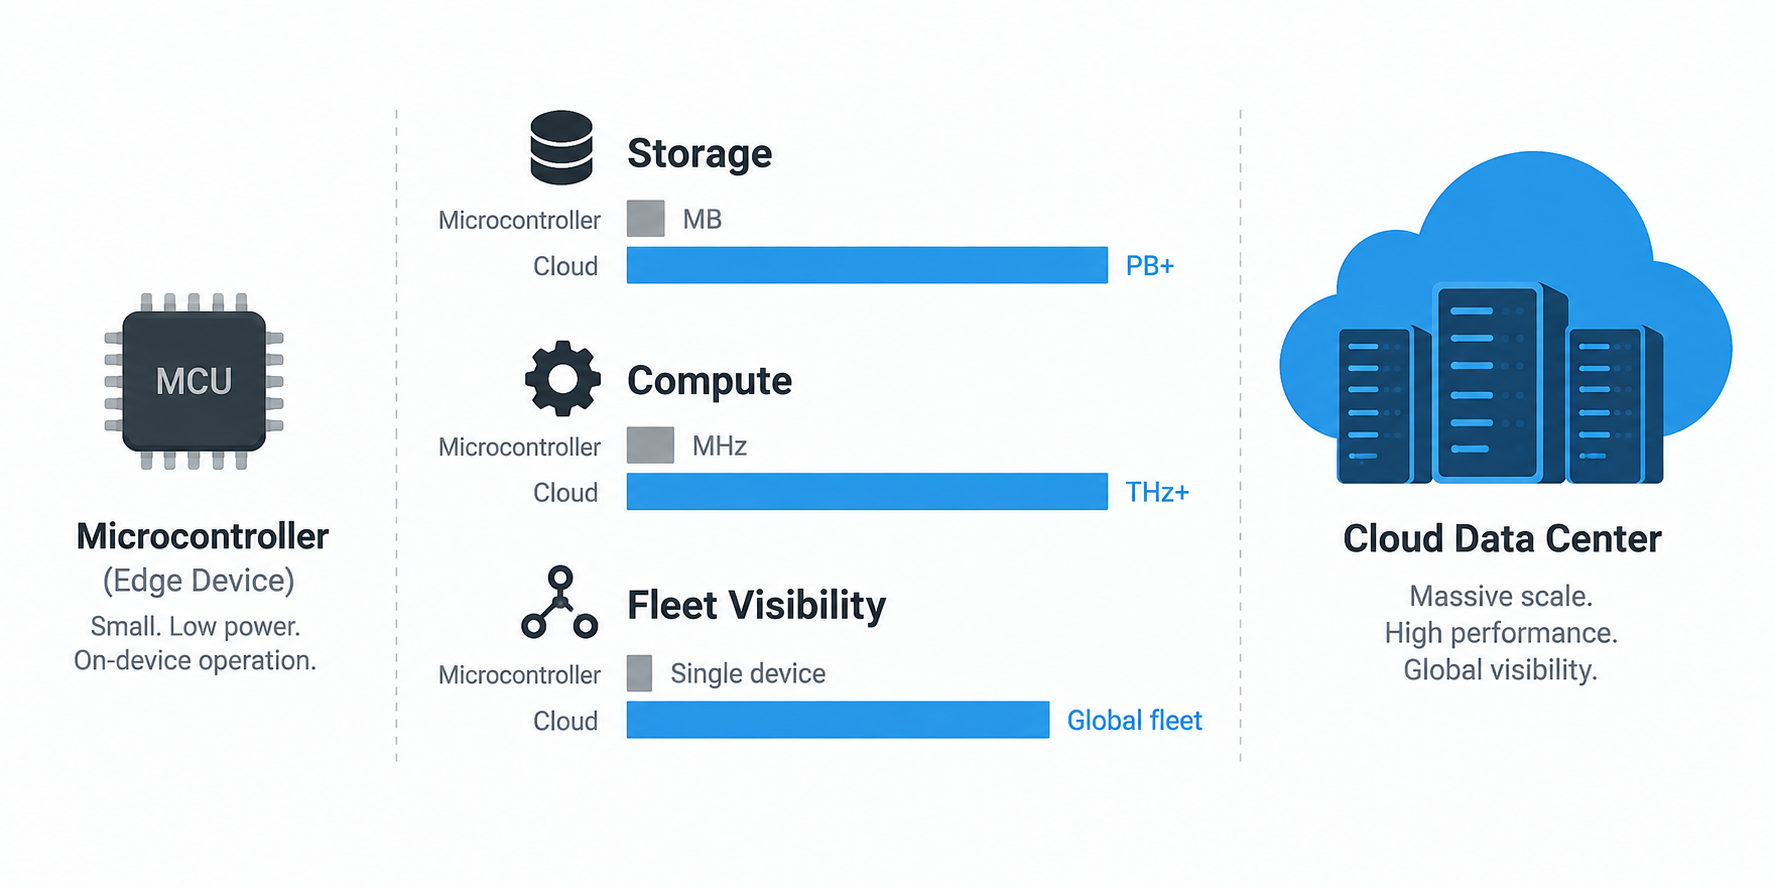
\includegraphics[width=0.9\textwidth]{lasttt-1.png}
\caption{Conceptual comparison of edge and cloud capabilities across the three motivating constraints.}
\label{fig:15_capability_comparison}
\end{figure}

% ============================================================
\section{The Concept of the Battery Digital Twin}
\label{sec:15_digital_twin}

A Digital Twin is not simply a static simulation model; it is a dynamic, living counterpart to a specific physical asset in the field. For a lithium-ion battery, the Digital Twin mirrors the physical pack's exact configuration, usage history, and environmental exposure.

\subsection{Architectural Components}
\label{subsec:15_architectural_components}

The Digital Twin architecture consists of three distinct pillars:
\begin{enumerate}
    \item \textbf{The Physical Asset:} The physical battery pack, equipped with voltage, current, and temperature sensors, managed by a lightweight Edge-BMS.
    \item \textbf{The Virtual Asset:} The cloud-hosted models. This includes electrochemical, equivalent circuit (ECM), and thermal models, as well as AI-driven degradation forecasters.
    \item \textbf{The Data Pipeline:} A bidirectional Internet-of-Things (IoT) telemetry link. It transmits raw sensor data up to the cloud and pushes updated parameter vectors and control limits down to the edge.
\end{enumerate}

By maintaining a synchronized virtual model, engineers can simulate "what-if" scenarios—such as the impact of a high-power fast-charging session on next week's capacity fade—without physically stressing the real battery.

\subsection{Fidelity Tiers of the Virtual Asset}
\label{subsec:15_fidelity_tiers}

Not every Digital Twin deployment operates at the same level of model fidelity, and production systems typically implement a tiered hierarchy rather than a single monolithic model, trading off computational cost against physical accuracy:

\begin{itemize}
    \item \textbf{Tier 1 — Equivalent Circuit Twin:} A cloud-hosted version of the same ECM used at the edge (Chapters~2–9), but re-fit periodically against the full historical telemetry record rather than only recent data, and unconstrained by the edge's real-time execution budget. This tier provides the most direct, explainable link back to the edge estimator and is typically used for routine parameter re-anchoring.
    \item \textbf{Tier 2 — Reduced-Order Electrochemical Twin:} A physics-based model (e.g., a Single Particle Model or reduced-order Doyle-Fuller-Newman formulation) capable of resolving internal concentration gradients and reaction kinetics that an ECM cannot represent, used primarily for deeper diagnostic investigation of anomalous cells flagged by Tier 1 or by the fleet analytics of Section~\ref{sec:15_fleet_analytics}.
    \item \textbf{Tier 3 — Data-Driven / Hybrid Twin:} The PINN and R-GCN architectures discussed in Section~\ref{sec:15_fleet_analytics}, which supplement or, in some deployments, substitute for the physics-based tiers when sufficient fleet data is available and physics-based models struggle to capture emergent, hard-to-model behaviors (such as manufacturing-defect-driven early failure signatures).
\end{itemize}

Running all three tiers continuously for every vehicle in a large fleet would itself be computationally and financially prohibitive at cloud scale; production deployments typically run Tier 1 continuously for every vehicle, and selectively escalate specific vehicles or cells to Tier 2 or Tier 3 analysis when Tier 1 residuals or fleet-level anomaly scores (Section~\ref{sec:15_fleet_analytics}) indicate that deeper investigation is warranted.

\subsection{Twin-Physical Synchronization and Divergence Monitoring}
\label{subsec:15_twin_sync}

A Digital Twin is only useful to the extent that it remains a faithful representation of its physical counterpart. Two related but distinct synchronization concerns must be managed:

\begin{itemize}
    \item \textbf{Update latency.} Because telemetry is aggregated and transmitted in batches (Section~\ref{sec:15_telemetry}) rather than streamed continuously, the twin's view of the vehicle is always at least somewhat stale — commonly by minutes for routine operational telemetry and, in bandwidth-constrained scenarios, by hours or longer. System designers must ensure that no safety-critical function is ever made contingent on twin freshness, reserving the twin strictly for functions where this inherent latency is acceptable (predictive maintenance, long-horizon SOH tracking) rather than functions requiring millisecond responsiveness (over-voltage protection).
    \item \textbf{Model-plant divergence.} Even with perfectly fresh data, the twin's internal model may gradually diverge from the true physical cell as unmodeled effects accumulate — a distinct phenomenon from the parameter drift the twin is trying to track, and closely related to the "silent model drift" concern raised in Chapter~15's discussion of fleet heterogeneity. Production Digital Twin platforms therefore continuously compute a \emph{residual score} between the twin's predicted terminal voltage and the physical vehicle's actually reported terminal voltage, and flag any vehicle whose residual exceeds a statistically-derived threshold for the Tier 2/Tier 3 escalation path described above, rather than assuming a low residual today guarantees a low residual indefinitely.
\end{itemize}

\begin{figure}[htbp]
\centering
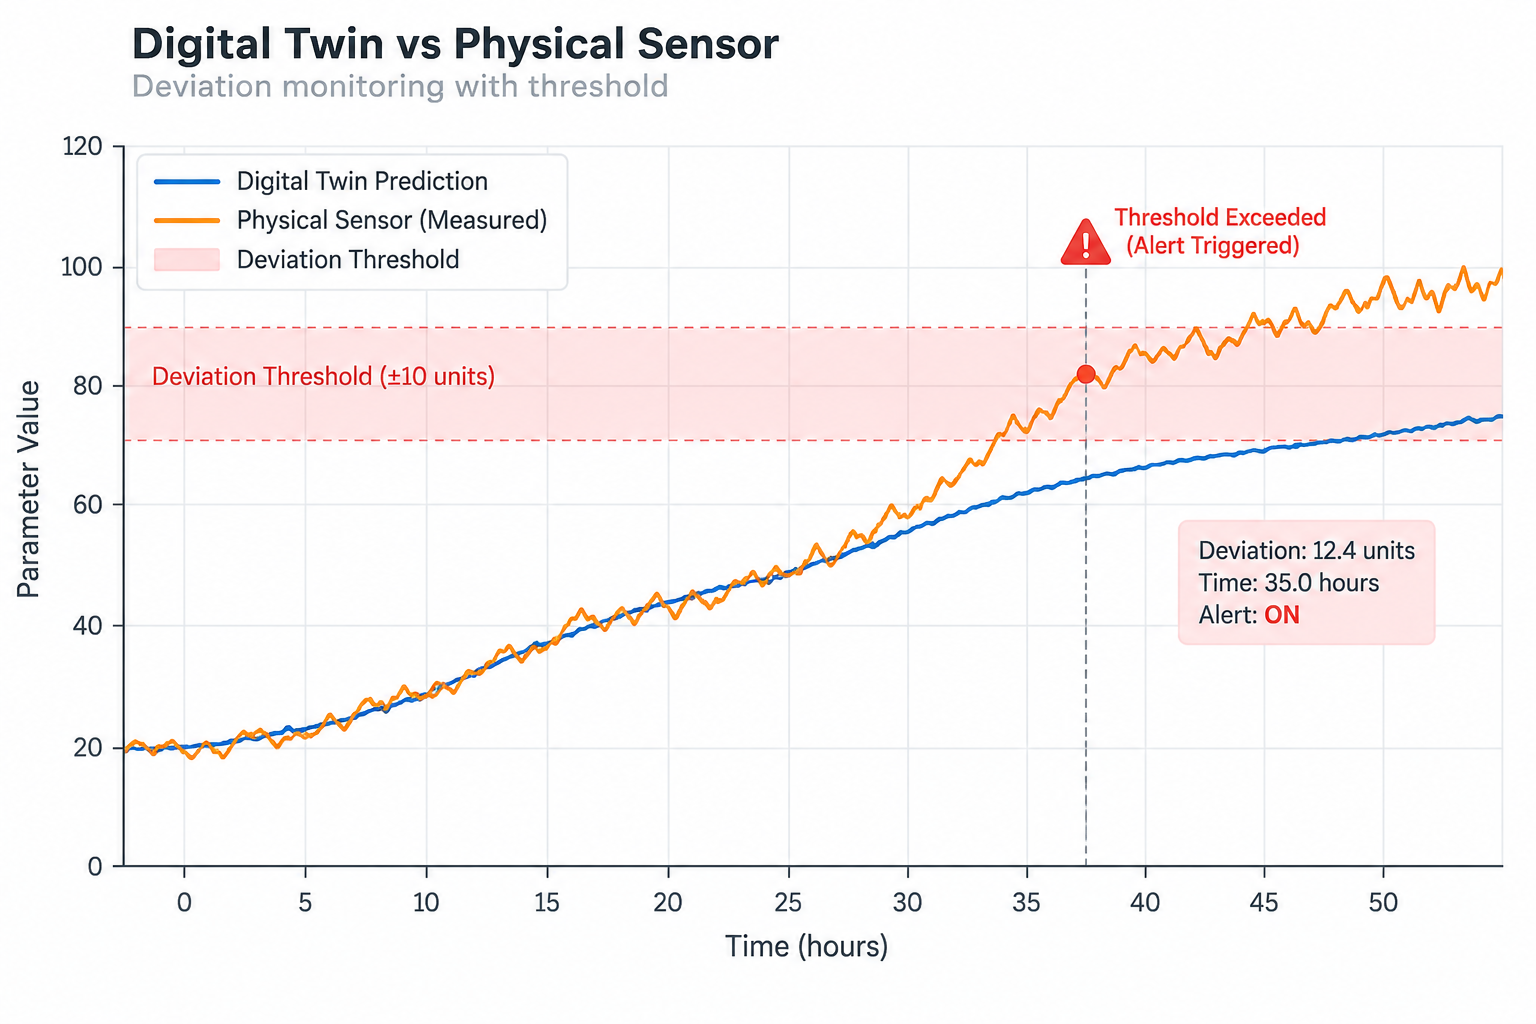
\includegraphics[width=0.9\textwidth]{last333.png}
\caption{Conceptual illustration of residual-based divergence monitoring between the Digital Twin and its physical counterpart.}
\label{fig:15_divergence_monitoring}
\end{figure}

% ============================================================
\section{IoT Telemetry and Data Pipelines}
\label{sec:15_telemetry}

Moving data from a moving vehicle to a cloud database introduces challenges regarding latency, bandwidth, and data integrity. It is impractical to stream 100~Hz data for 100 individual cells continuously over a cellular network.

\subsection{Edge Data Aggregation}
\label{subsec:15_edge_aggregation}

Instead of raw streaming, the Edge-BMS acts as an intelligent aggregator. Using lightweight IoT microcontrollers, the edge system buffers high-frequency data, performs basic anomaly detection, and compresses the telemetry. The data is packaged into structured payloads and transmitted via protocols like MQTT (Message Queuing Telemetry Transport) to backend servers.

\subsection{Bandwidth Budgeting}
\label{subsec:15_bandwidth}

Table~\ref{tab:15_bandwidth_budget} illustrates why raw, unaggregated per-cell streaming is impractical at fleet scale, and motivates the compression and summarization strategies discussed below.

\begin{table}[htbp]
\centering
\footnotesize
\caption{Bandwidth for a 96-cell pack via different strategies.}
\label{tab:15_bandwidth_budget}
\renewcommand{\arraystretch}{1.2}
\begin{tabularx}{\columnwidth}{@{} >{\raggedright\arraybackslash}X >{\raggedright\arraybackslash}X >{\raggedright\arraybackslash}X @{}}
\toprule
\textbf{Strategy} & \textbf{Data Rate} & \textbf{Feasibility} \\
\midrule
Raw per-cell (100~Hz) & $\sim$Mbps/veh & Infeasible on cellular. \\
Pack aggregate (1~Hz) & $\sim$10s B/s & Feasible (standard). \\
Event-triggered bursts & Short duration & Feasible (diagnostics). \\
Overnight full upload & Large batch & Feasible (via Wi-Fi). \\
\bottomrule
\end{tabularx}
\end{table}

\subsection{Protocol Selection}
\label{subsec:15_protocol}

MQTT is the dominant protocol choice for vehicle-to-cloud telemetry due to its lightweight publish/subscribe model, small message-header overhead relative to alternatives such as HTTP, and native support for configurable quality-of-service levels, allowing the Edge-BMS to specify, on a per-message basis, whether a given payload merits guaranteed delivery (e.g., a fault event) or best-effort delivery (e.g., routine telemetry that will simply be superseded by the next periodic update if lost). Constrained Application Protocol (CoAP) is sometimes used as an alternative in deployments prioritizing even lower overhead over MQTT's broker-mediated flexibility, particularly in narrowband IoT (NB-IoT) connectivity scenarios with severely constrained data budgets.

\subsection{Store-and-Forward Reliability}
\label{subsec:15_store_forward}

Vehicles routinely traverse regions of degraded or absent cellular connectivity (tunnels, parking garages, rural areas), meaning the telemetry pipeline cannot assume a continuously available network link. Production Edge-BMS telemetry stacks therefore implement a local store-and-forward buffer: aggregated payloads are queued locally (typically in a small circular buffer sized to hold several hours to a few days of aggregated data) and transmitted opportunistically as connectivity becomes available, with the buffer's overwrite policy carefully designed to preserve diagnostically significant events (fault flags, anomaly-triggered bursts) preferentially over routine telemetry if the buffer fills before connectivity is restored.

\subsection{Backend Database Integration}
\label{subsec:15_backend_db}

Once the data reaches the cloud, it is routed into scalable backend databases (e.g., time-series databases or managed platforms utilizing PostgreSQL). This continuous ingestion builds a massive historical repository for each vehicle. Because cloud databases support rapid query execution and seamless integration with AI frameworks like PyTorch or TensorFlow, the heavy lifting of data preprocessing and feature extraction (such as the Incremental Capacity peaks from Chapter~13) is handled entirely off-board.


% ============================================================
\section{Computational Partitioning: Edge vs. Cloud}
\label{sec:15_partitioning}

A successful Cloud-BMS does not replace the local BMS; it augments it. The responsibilities must be strictly partitioned based on latency requirements and safety criticality.

\begin{table}[htbp]
\centering
\footnotesize
\caption{Task partitioning in a Cloud-BMS architecture.}
\label{tab:15_edge_vs_cloud}
\renewcommand{\arraystretch}{1.3}
% Adjusted for narrow/two-column layouts. Adjust the cm values if needed.
\begin{tabular}{@{} l p{3cm} p{3.2cm} @{}}
\toprule
\textbf{Function} & \textbf{Edge-BMS (Local)} & \textbf{Cloud-BMS (Twin)} \\
\midrule
\textbf{State Est.} & Fast SOC/$U_p$ via EKF. & Historic SOC smoothing. \\
\textbf{Param. ID} & Instant $R_0$ tracking. & Weekly aging ($Q_n$, SEI) ID. \\
\textbf{Safety} & Hardware thermal cutoffs. & Predictive anomaly alerts. \\
\textbf{Balancing} & Executes HW balancing. & Computes optimal targets. \\
\bottomrule
\end{tabular}
\end{table}
\subsection{A Latency-Driven Decision Framework}
\label{subsec:15_latency_framework}

Rather than partitioning functions on an ad hoc, case-by-case basis, production architects generally apply a simple governing rule: \emph{any function whose failure or delay could contribute to an unsafe condition within the vehicle's fault-tolerant time interval must reside entirely on the edge, with no dependency on cloud connectivity.} The fault-tolerant time interval — the maximum time a safety-relevant condition can persist before it must be mitigated — is typically on the order of tens to hundreds of milliseconds for electrical safety functions (over-voltage, over-current) and seconds for thermal functions, both far shorter than any achievable cloud round-trip latency over a cellular network, which routinely spans hundreds of milliseconds to seconds even under good connectivity and is unbounded under poor or absent connectivity. This rule directly explains the partitioning shown in Table~\ref{tab:15_edge_vs_cloud}: state estimation and safety controls remain edge-resident specifically because their fault-tolerant time intervals are shorter than achievable cloud latency, while parameter identification and predictive maintenance are cloud-eligible specifically because their relevant timescales (days to weeks) comfortably exceed any realistic telemetry and processing delay.

\subsection{Hybrid Ownership: Balancing Target Computation}
\label{subsec:15_hybrid_ownership}

The balancing row of Table~\ref{tab:15_edge_vs_cloud} deserves particular attention as an illustration of genuinely hybrid task ownership. The Edge-BMS retains full authority over \emph{execution} of balancing hardware (Chapter~14) — closing bleed-resistor switches or driving active-balancing converters — since this is a real-time, safety-adjacent actuation function. However, the cloud-side Digital Twin can compute improved balancing \emph{targets}, informed by long-horizon thermal-gradient history (Chapter~14, Section~14.2) that no single charge cycle's edge-local data could reveal — for example, recognizing that a specific brick position has consistently run hot across the vehicle's entire service history and pre-biasing its target SOC slightly lower heading into each charge event, rather than reacting only to the current charge cycle's measured imbalance. This division — cloud computes strategy, edge executes tactics — recurs as a template across several of the hybrid functions discussed later in this chapter.

% ============================================================
\section{Cloud-Based AI and Fleet Analytics}
\label{sec:15_fleet_analytics}

The most significant advantage of the Cloud-BMS is the ability to view the battery not in isolation, but as part of a fleet.

\subsection{Deploying Advanced AI Models}
\label{subsec:15_deploying_ai}

As discussed in Chapter~12, models like Physics-Informed Neural Networks (PINNs) require significant processing power to compute gradient penalties based on thermodynamic equations. The cloud provides the ideal environment for these models. Telemetry data feeds the PINN, which predicts the battery's core temperature and aging trajectory.

Furthermore, by applying Relational Graph Convolutional Networks (R-GCNs) on the cloud side, the Digital Twin can model the entire pack topology. The R-GCN processes the electrical and thermal relationships between individual cells as graph edges, predicting how a localized hotspot will propagate and degrade neighboring cells over the coming months.

\subsection{Fleet-Wide Anomaly Detection}
\label{subsec:15_fleet_anomaly}

Beyond per-vehicle modeling, aggregating telemetry across an entire fleet enables a distinct class of analysis unavailable to any single vehicle's edge controller: population-relative anomaly detection. Rather than asking "is this cell behaving abnormally relative to its own history," the fleet analytics layer can ask "is this cell, or this vehicle, behaving abnormally relative to thousands of comparable cells and vehicles under similar conditions" — a substantially more sensitive test, particularly for detecting slow-onset manufacturing defects that would appear unremarkable against a single vehicle's own history but stand out clearly against a large, statistically well-characterized population baseline. This population-relative approach is a primary mechanism by which fleet operators identify candidate battery recalls or targeted service campaigns well before individual vehicle owners would notice any perceptible performance change.

\subsection{Federated Learning}
\label{subsec:15_federated_learning_full}

When a single vehicle experiences a rare stress event (e.g., rapid degradation due to sub-zero fast charging), the cloud model updates its understanding of that degradation mechanism. Through \textbf{Federated Learning} or centralized model updating, this newly acquired intelligence is generalized and pushed via Over-The-Air (OTA) updates to the entire fleet. Consequently, Vehicle B can preemptively adjust its charging limits to avoid the degradation observed in Vehicle A, even if Vehicle B has never experienced those harsh conditions.

It is worth distinguishing the two update strategies referenced above, as they carry different privacy and bandwidth trade-offs. \textbf{Centralized model updating} transmits raw or lightly-processed telemetry from every vehicle to the cloud, where a single model is retrained directly against the pooled dataset — simpler to implement and reason about, but requiring that potentially sensitive usage data leave the vehicle in a relatively raw form. \textbf{Federated learning} instead trains a local model increment on each vehicle's own edge or regional-gateway hardware and transmits only the resulting model-weight updates (or gradients) back to a central aggregator, which combines updates from many vehicles into a single improved global model without any single vehicle's raw telemetry ever leaving that vehicle. The federated approach directly addresses the data-privacy and bandwidth concerns of centralized updating, at the cost of a more complex aggregation protocol and, typically, slower convergence than training directly against a fully centralized dataset.

\subsection{Deployment Pipelines: Canary Rollout and A/B Validation}
\label{subsec:15_canary}

Regardless of which update strategy produces the improved model, pushing that model — or an updated parameter vector derived from it — back down to a live vehicle fleet via OTA update is itself a high-stakes engineering step, since an erroneous update deployed uniformly across an entire fleet could simultaneously degrade the performance or safety margins of every vehicle that receives it. Production Cloud-BMS platforms mitigate this risk through staged \textbf{canary rollout}: a new model or parameter update is first deployed to a small, carefully monitored subset of the fleet (the "canary" population), its real-world performance is compared against a held-out control group still running the previous model (an A/B validation comparison), and only after the canary population demonstrates statistically significant improvement without any safety-relevant regression is the update progressively rolled out to the broader fleet. This staged deployment discipline is analogous to canary and blue-green deployment practices common in conventional cloud software engineering, adapted here to the higher-stakes context of a safety-relevant embedded system.



% ============================================================
\section{Security Architecture for the Cloud-BMS Pipeline}
\label{sec:15_security}

Because the Cloud-BMS pipeline described in this chapter establishes a bidirectional data channel with direct influence over a safety-relevant embedded system, it must be treated as a security-critical system in its own right, not merely a convenience feature layered on top of the estimation architectures of earlier chapters.

\subsection{Threat Model}
\label{subsec:15_threat_model}

At minimum, the pipeline must defend against three broad threat categories: (1) \emph{interception and tampering} of telemetry or parameter-update payloads in transit between vehicle and cloud; (2) \emph{spoofing}, in which an attacker injects fabricated telemetry or a fraudulent parameter update impersonating a legitimate cloud endpoint or vehicle; and (3) \emph{rollback attacks}, in which an attacker forces a vehicle to revert to an older, known-vulnerable firmware or parameter set after a security fix has already been deployed.

\subsection{Mitigations}
\label{subsec:15_mitigations}

Standard mitigations, drawn from established automotive and IoT security practice, include end-to-end transport encryption (typically TLS) combined with message-level cryptographic signing of every parameter update, so that the vehicle can verify both the authenticity and integrity of an update independent of the transport layer's own security; a hardware root-of-trust and secure boot chain on the vehicle-side microcontroller, ensuring that only signed, verified firmware and parameter payloads are ever accepted for execution; and monotonic version enforcement, in which the vehicle refuses to install any update bearing a version identifier older than its currently installed version, directly closing the rollback-attack vector described above.


% IMAGE PROMPT: A clean, technical cybersecurity infographic showing a padlock icon over a data stream flowing between a stylized electric vehicle icon and a cloud server icon, with small badge icons representing "Encrypted", "Signed", and "Version-Checked" along the connection. Minimalist, dark navy background, white and cyan line-art style, automotive cybersecurity aesthetic.

% ============================================================
\section{Case Study: End-to-End Predictive Maintenance Flow}
\label{sec:15_case_study}

To ground the architectural concepts of this chapter in a concrete scenario, consider a representative predictive-maintenance flow as it would unfold across the Cloud-BMS pipeline described above:

\begin{enumerate}
    \item \textbf{Routine telemetry.} A vehicle's Edge-BMS aggregates 1~Hz pack-level bar-and-delta summaries (Chapter~14) throughout a normal driving day and transmits them via MQTT during the next available connectivity window, per Section~\ref{subsec:15_edge_aggregation}.
    \item \textbf{Tier 1 twin update.} The cloud-hosted equivalent-circuit twin (Section~\ref{subsec:15_fidelity_tiers}) ingests the new telemetry and re-anchors its slow parameter estimates, computing an updated residual score as described in Section~\ref{subsec:15_twin_sync}.
    \item \textbf{Fleet-relative anomaly flag.} The fleet analytics layer (Section~\ref{subsec:15_fleet_anomaly}) observes that one specific brick in this vehicle's pack shows a resistance-growth trajectory in the top 1\% of a large population of comparable vehicles, despite no single edge-local threshold having been crossed.
    \item \textbf{Escalation to Tier 2/3 analysis.} Because the anomaly score exceeds the escalation threshold, the flagged cell's full telemetry history is routed to the reduced-order electrochemical and R-GCN models (Sections~\ref{subsec:15_fidelity_tiers} and~\ref{subsec:15_fleet_analytics}) for deeper diagnostic evaluation, which estimates a specific, elevated probability of accelerated LAM-driven fade (Chapter~13) over the coming months.
    \item \textbf{Actionable output.} The Digital Twin platform generates a predictive-maintenance recommendation — for example, adjusting the vehicle's default charging current limit slightly downward to reduce further stress on the flagged brick, or notifying the fleet operator to schedule a service inspection — which is pushed back to the vehicle through the secure, canary-validated OTA pipeline of Sections~\ref{subsec:15_canary} and~\ref{sec:15_security}.
\end{enumerate}

This flow illustrates, end to end, how the individually-described components of this chapter — telemetry aggregation, tiered digital-twin modeling, fleet-relative analytics, secure staged deployment — combine into a single coherent capability that no edge-only architecture from earlier chapters could provide in isolation.

% ============================================================
\section{Summary}
\label{sec:15_summary}

The Cloud-BMS and Digital Twin architecture represents the final frontier of battery parameter estimation. By breaking free from the computational constraints of embedded edge hardware, engineers can deploy massive, data-driven AI models—including PINNs and pack-level R-GCNs—to track slow-moving degradation mechanics with unprecedented accuracy. The edge handles the millisecond-level safety and transient tracking, while the cloud handles the predictive analytics, storing entire lifetimes of telemetry in scalable backend databases, structured across fidelity tiers that balance model richness against computational cost. A disciplined latency-driven partitioning framework, robust store-and-forward telemetry pipelines, fleet-relative anomaly detection, privacy-preserving federated learning, staged canary deployment, and end-to-end cryptographic security together ensure that this cyber-physical synergy improves battery performance and longevity without compromising the safety guarantees that must remain the exclusive responsibility of the edge. Together, this architecture ensures that battery packs operate safely, adapt continuously to user behavior, and achieve their maximum theoretical lifespan.

% ============================================================


% ============================================================
% ARCHITECTURE DIAGRAM PLACEHOLDER
% ============================================================
\begin{figure}[htbp]
    \centering
    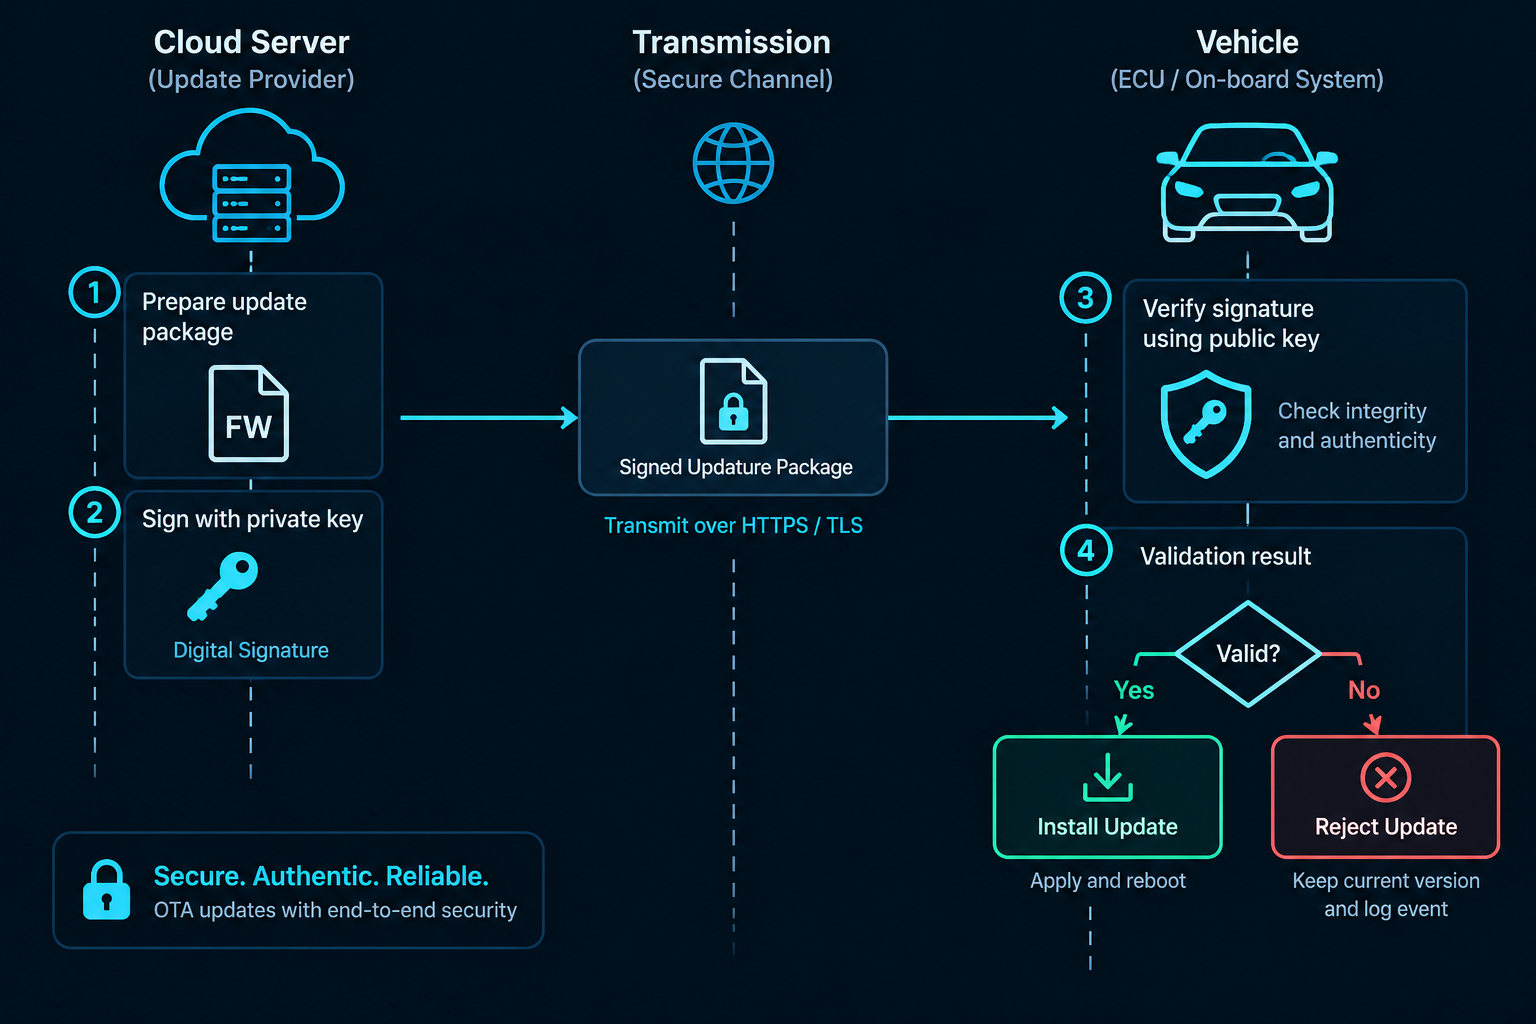
\includegraphics[width=0.9\textwidth]{lastfinal.png}
  

  
  
    \caption{Bidirectional architecture dividing fast-transient safety controls at the edge and computationally heavy AI/aging analytics in the cloud.}
    \label{fig:15_cloud_architecture}
\end{figure}

% ============================================================
% AI IMAGE GENERATION PROMPTS
% ============================================================
% PROMPT 1 (For Section 15.1 - Edge vs Cloud Capability Comparison):
% "A clean, minimalist infographic comparing a small microcontroller chip 
% icon against a large cloud data-center icon, with three labeled bar-chart 
% metrics between them: 'Storage', 'Compute', and 'Fleet Visibility', 
% showing the cloud icon vastly larger on each metric. Flat vector style, 
% blue and gray corporate technical-report palette."
%
% PROMPT 2 (For Section 15.2.3 - Twin-Physical Divergence Monitoring):
% "A technical line-chart illustration showing two overlapping curves — 
% a smooth 'digital twin prediction' line in blue and a slightly noisier 
% 'physical sensor' line in orange — gradually diverging over a time axis, 
% with a shaded threshold band and a small alert icon where the gap crosses 
% the threshold. Clean engineering dashboard style."
%
% PROMPT 3 (For Section 15.3 - Telemetry Data Pipeline):
% "A horizontal flow-diagram illustration showing icons connected by arrows: 
% a car with sensor icons, a small buffer/queue icon, a cloud upload icon, 
% a database cylinder icon, and a neural network icon at the end. Flat 
% vector infographic style, muted blue and teal palette, IoT architecture 
% aesthetic."
%
% PROMPT 4 (For Section 15.5 - Canary Rollout Funnel):
% "A funnel-shaped infographic illustration showing a software update icon 
% at the top narrowing through stages labeled '1% Canary', '10%', '50%', 
% '100% Fleet', with a small red rollback arrow curling back from each 
% stage to the top. Clean SaaS-dashboard illustration style, green and 
% amber color accents indicating pass/fail gates."
%
% PROMPT 5 (For Section 15.6 - Secure OTA Update Sequence):
% "A technical sequence-diagram-style illustration showing a cloud server 
% icon signing a small padlocked data package, which is transmitted to a 
% vehicle icon that checks it against a key/shield icon before an 'Install' 
% or 'Reject' outcome. Minimalist cybersecurity vector illustration, dark 
% background, cyan and white accent lines."
% ============================================================